\documentclass[aspectratio=169]{beamer}
\usepackage[scaled]{helvet}
\usepackage[utf8]{inputenc}
\usepackage{amssymb,amsmath,amsfonts}
\usepackage{natbib}
\usepackage{smartdiagram}

\usetheme{ifors}

\bibliographystyle{plain}

\title{\textbf{Optimization models for crime analytics applied to social networks}}
\author{\textbf{Richard Weber}\inst{a} \and Fredy Troncoso\inst{b} \and Alex Barrales-Araneda\inst{b}}
\institute{%
\inst{a}{Department of Industrial Engineering, FCFM, University of Chile} 
\inst{b}{Department of Industrial Engineering, University of Bío-Bío}
}

\date{July 10, 2022. Santiago, Chile}

\renewcommand\familydefault{\sfdefault}

\begin{document}

\begin{frame}
  \setbeamertemplate{footline}{}
  \titlepage
\end{frame}

\begin{frame}
  \frametitle{Outline}
  \tableofcontents
\end{frame}

\section{Introduction}
\subsection{Introduction}
\begin{frame} 
\frametitle{Introduction}
  \begin{columns}
  \column{0.5\textwidth}
    \begin{enumerate} 
      \item Criminal investigation usually involves the mobilization of large amounts of human and technical resources in search of persons responsible for a crime.
      \item Knowledge about the structure and organization of criminal networks is important both for investigation and for the development of effective crime prevention strategies\cite{Xu2005}.
    \end{enumerate}
  \column{0.5\textwidth}
    \centering
    \includegraphics[width=0.65\textwidth]{images/band.png}
  \end{columns}
\end{frame}

\subsection{Criminal networks}

\begin{frame}
\frametitle{Criminal networks}
  \begin{columns}
  \column{0.5\textwidth}
    \begin{enumerate}
      \item A criminal group can be understood as a social network in which the nodes represent the suspects and the arcs are the links between individuals.
      \item These links act as channels for the transfer or flow of material and/or immaterial resources. \cite{Mci99}
    \end{enumerate}
  \column{0.5\textwidth}
    \centering
    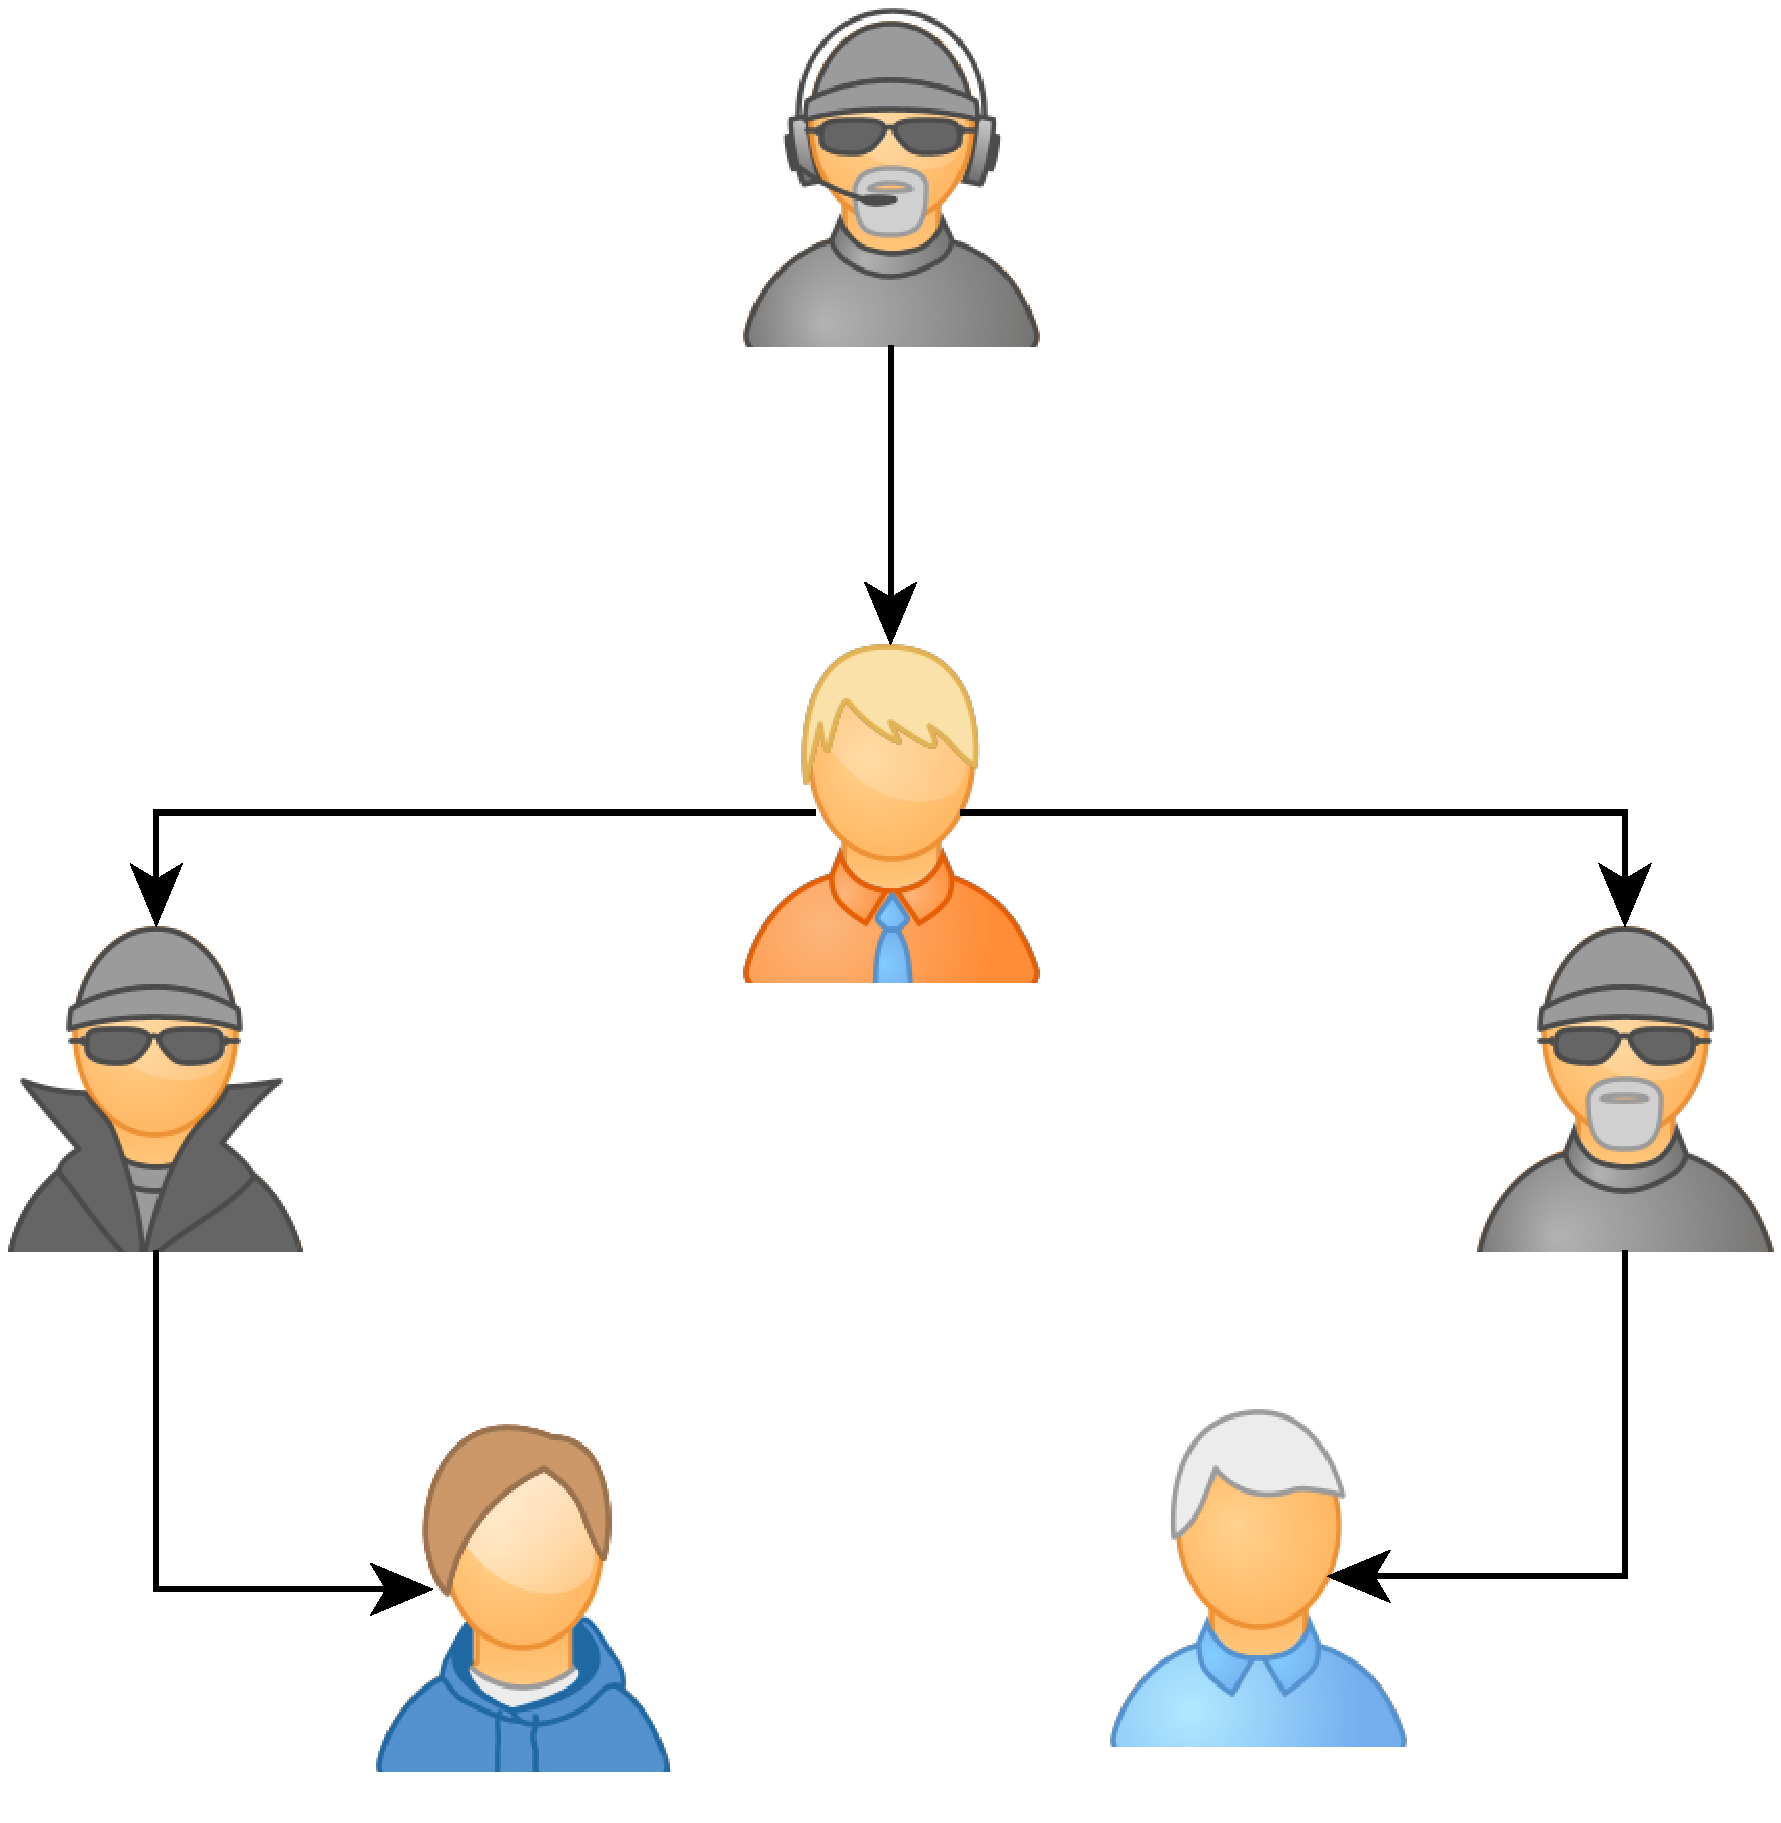
\includegraphics[width=0.9\textwidth]{images/CG.pdf}
  \end{columns}
\end{frame}

\subsection{Extraction of information from social networks}
\begin{frame}
\frametitle{Extraction of information from social networks}
  \begin{columns}
  \column{0.5\textwidth}
    \begin{enumerate}
      \item There are two approaches to extracting information from social networks: the evaluation of important individuals and the identification of associations.
      \item The main evaluators of individuals are derived from Social Network Analysis (SNA). \cite{Mci99}.
      \item The techniques for identifying associations present in the literature are based on relationships between individuals (SPA).
    \end{enumerate}
  \column{0.5\textwidth}
    \smartdiagram[priority descriptive diagram]{
      {Evaluation of important individuals},
      {Identification of associations based on relationships},
      {Identification of associations based on $pcg$.}
    }
  \end{columns}
\end{frame}

\section{Identification of associations based on optimization models}
\subsection{Network preparation}
\begin{frame}
\frametitle{Propensity to belong to a criminal group}
  \begin{columns}
  \column{0.5\textwidth}
    \begin{enumerate}
      \item The indicator $pcg_i$ is introduced as the propensity of each individual $i \in N$ to belong to a criminal group.
      \item The general form of estimating $pcg_i$ is given by:
      \begin{equation*}
        pcg_i = f(s_i), \forall i \in N
      \end{equation*}
      where $s_i$ is the set of relevant attributes of individual $i$, and $f$ is some function that transforms these attributes into a propensity score.
    \end{enumerate}
  \column{0.5\textwidth}
    \begin{figure}[ht]
      \centering
      \includegraphics[width=\textwidth]{images/decision-tree.png}
    \end{figure}
  \end{columns}
\end{frame}

\begin{frame}
\frametitle{Network preparation}
  \begin{columns}
  \column{0.5\textwidth}
    \begin{enumerate}
      \item Criminal skills are represented by the criminal propensity $pcg$ and trust is represented by the social distance between individuals $d_{ij}$.
      \item The social distance between two individuals is represented by a value between $0$ and $1$, where $1$ represents the maximum distance between them.
      \item We define an arc when there is a common crime between a pair of individuals.
    \end{enumerate}
  \column{0.5\textwidth}
    \begin{figure}[ht]
      \centering
      \includegraphics[width=\textwidth]{images/network.png}
    \end{figure}
  \end{columns}
\end{frame}

\subsection{Linear rational association model (LiRAM)}

\begin{frame}
\frametitle{Linear rational association model (LiRAM)}
  \begin{columns}
  \column{0.5\textwidth}
    \begin{enumerate}
      \item<1-> The search for the best association can be interpreted as the process of forming a criminal group in which a planner chooses individuals to participate based on their criminal capabilities and reliability, maximizing some utility function.
      \item<2-> The LiRAM model determines the subset of individuals $i \in N$ and the set of arcs $(i,j) \in A$ that form the best association between individuals $s$ (planner) and $d$ (receiver).
    \end{enumerate}
  \column{0.5\textwidth}
    \begin{figure}[ht]
      \centering
      \only<1> {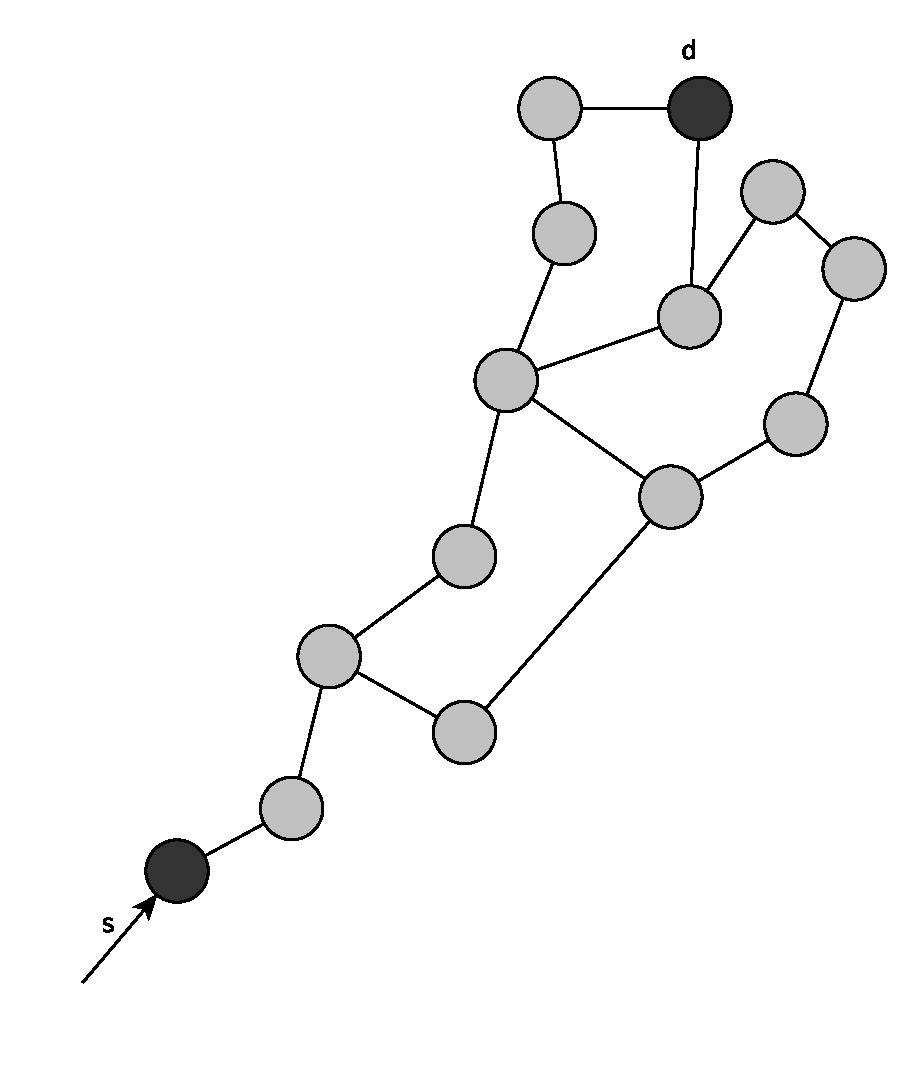
\includegraphics[width=0.7\textwidth]{images/liram-1.pdf}}%\caption{Figure ?}}
      \only<2->{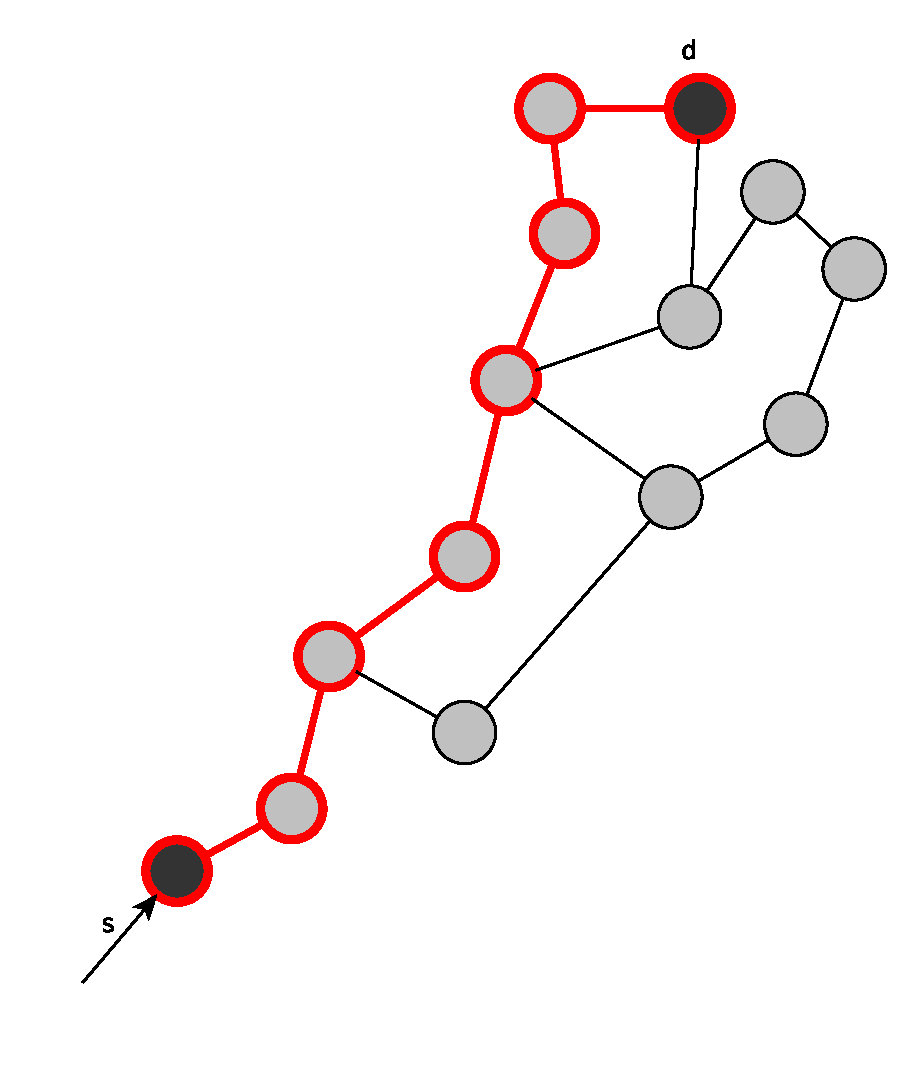
\includegraphics[width=0.7\textwidth]{images/liram-2.pdf}}%\caption{Figure ?}}
    \end{figure}
  \end{columns}
\end{frame}

\begin{frame}
\frametitle{Linear rational association model (LiRAM)}
\begin{columns}
  \column{0.6\textwidth}
    \begin{block}{Decision variables}
    \footnotesize
      \vspace{1em}
      $y_{i} =
        \begin{cases}
          1 & \text{if $i \in N$ is in the criminal group}\\
          0 & \text{otherwise}
        \end{cases}$\\
      $x_{ij} =
        \begin{cases}
          1 & \text{if $(i,j) \in A$ is in the solution}\\
          0 & \text{otherwise}
        \end{cases}$
    \end{block}
  \begin{block}{Objective function}
    \begin{itemize}
    \footnotesize
      \item Utility function of a crime planner.
      \begin{equation*}
        \max U = \frac{I}{pcg_{max}} \sum_{i \in N} pcg_i y_i - \frac{I \gamma}{d_{max}} \sum_{(i,j) \in A} d_{ij} x_{ij} - w \sum_{i \in N} pcg_i y_i
      \end{equation*}
    \end{itemize}
  \end{block}
  \column{0.4\textwidth}
    \begin{figure}[ht]
      \centering
      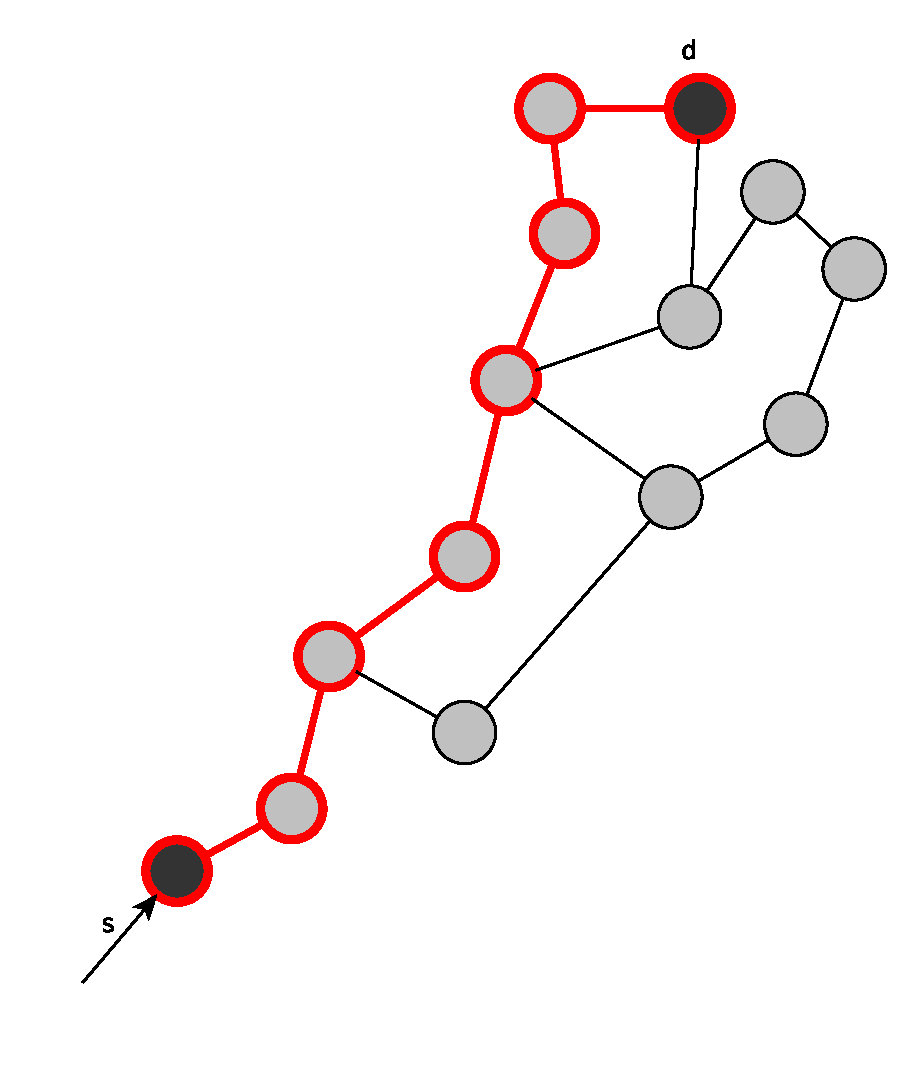
\includegraphics[width=0.7\textwidth]{images/liram-2.pdf}
    \end{figure}
  \end{columns}
\end{frame}

\begin{frame}
\frametitle{Linear rational association model (LiRAM)}
\begin{block}{Constraints}
  \begin{scriptsize}
    \begin{columns}[t]
      \column{0.46\textwidth}
      \begin{itemize}
        \item Predecessor constraint:
        \begin{align}
          & \sum_{i \in N} x_{ij} = y_{j} & \forall j \in N \setminus \{s, d \} \\
          \intertext{\item Flow conservation:}
          & \sum_{i \in N} x_{ij} = \sum_{i \in N} x_{ji} & \forall j \in N \setminus \{s, d \} \\
          \intertext{\item Maximum criminal propensity:}
          & \sum_{i \in N} pcg_i y_i \leq \varphi pcg_{max}
        \end{align}
      \end{itemize}
      \column{0.54\textwidth}
      \begin{itemize}
        \item Subtour elimination constraints:
        \begin{align}
          & \sum_{i,j \in L} x_{ij} = |L| - 1 & \forall L \subseteq N \setminus \{s, d \}: |L| \geq 2 \\
          \intertext{\item Initial and final flow:}
          & \sum_{j \in N} x_{sj} = \sum_{i \in N} x_{id} = 1 \\
          \intertext{\item Variable’s domain:}
          & x_{ij} \in \{0,1\} &\forall (i,j) \in A \\
          & y_{i} \in \{0,1\} &\forall i \in N
        \end{align}
      \end{itemize}
      \vfill
    \end{columns}
  \end{scriptsize}
\end{block}
\end{frame}

\subsection{Steiner tree rational association model (StRAM)}
\begin{frame}
\frametitle{Steiner tree rational association model (StRAM)}
  \begin{columns}
  \column{0.5\textwidth}
    \begin{enumerate}
      \item<1-> The planner is rational and chooses criminals with the skills that will ensure that the crime is carried out with the maximum utility.
      \item<2-> The StRAM model determines the Steiner tree, rooted in the crime planner $s \in N$.
      \item<3-> Requires a single suspect to determine criminal groups
    \end{enumerate}
  \column{0.5\textwidth}
    \begin{figure}[ht]
      \centering
      \includegraphics[width=\textwidth]{images/stram-network.pdf}
    \end{figure}
  \end{columns}
\end{frame}

\begin{frame}
\frametitle{Steiner tree rational association model (StRAM)}
\begin{columns}
  \column{\textwidth}
    \begin{block}{Decision variables}
    \footnotesize
      \vspace{1em}
      $y_{i} =
        \begin{cases}
          1 & \text{if $i \in N$ is in the criminal group}\\
          0 & \text{otherwise}
        \end{cases}$\\
      $x_{ij} =
        \begin{cases}
          1 & \text{if $(i,j) \in A$ is in the solution}\\
          0 & \text{otherwise}
        \end{cases}$\\
      $f_{ij} = \text{flow through the arc $(i,j) \in A$}$
    \end{block}
  \begin{block}{Objective function}
    \begin{itemize}
    \footnotesize
      \item Utility function of a crime planner
      \begin{equation*}
        \max U = \frac{I}{pcg_{max}} \sum_{i \in N} pcg_i y_i - \frac{I \gamma}{d_{max}} \sum_{(i,j) \in A} d_{ij} x_{ij} - w \sum_{i \in N} pcg_i y_i
      \end{equation*}
    \end{itemize}
  \end{block}
  \end{columns}
\end{frame}

\begin{frame}
\frametitle{Steiner tree rational association model (StRAM)}
\begin{block}{Constraints}
  \begin{scriptsize}
    \begin{columns}[t]
      \column{0.5\textwidth}
      \begin{itemize}
        \item Predecessor constraint:
        \begin{align}
          & \sum_{i \in N} x_{ij} = y_{j} & \forall j \in N \setminus \{s\} \\
          \intertext{\item Flow conservation:}
          & \sum_{i \in N} f_{ij} - \sum_{i \in N} f_{ji} = y_{j} & \forall j \in N \setminus \{s\} \\
          \intertext{\item Link of the variables:}
          & f_{ij} \leq (|N| - 1) x_{ij} & \forall (i,j) \in A
        \end{align}
      \end{itemize}
      \column{0.5\textwidth}
      \begin{itemize}
        \item Maximum criminal propensity:
        \begin{align}
          & \sum_{i \in N} pcg_i y_i \leq \varphi pcg_{max}\\
          \intertext{\item Variable’s domain:}
          & f_{ij} \geq 0 &\forall (i,j) \in A \\
          & x_{ij} \in \{0,1\} &\forall (i,j) \in A \\
          & y_{i} \in \{0,1\} &\forall i \in N
        \end{align}
      \end{itemize}
      \vfill
    \end{columns}
  \end{scriptsize}
\end{block}
\end{frame}

\subsection{New criminal association model based on Steiner tree (NCAM)}
\begin{frame}
\frametitle{New criminal association model based on Steiner tree (NCAM)}
  \begin{columns}
  \column{0.5\textwidth}
    \begin{enumerate}
      \item<1-> The total social capital of the group is maximized, considering that interactions allow sharing part of the knowledge.
      \item<2-> Allows to generate results in networks where there are no known suspects.
    \end{enumerate}
  \column{0.5\textwidth}
    \begin{figure}[ht]
      \centering
      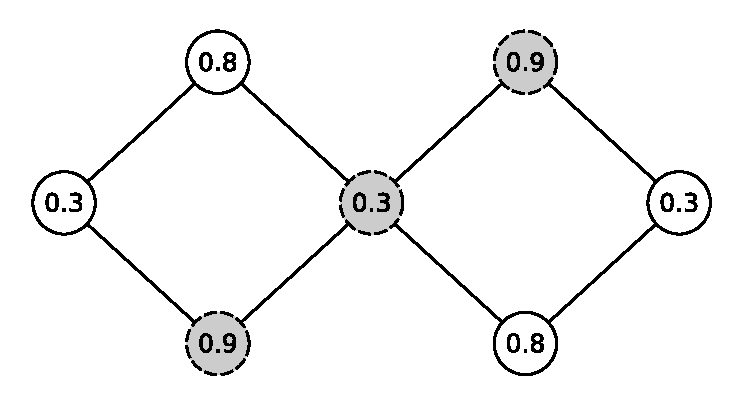
\includegraphics[width=\textwidth]{images/ncam.pdf}
    \end{figure}
  \end{columns}
\end{frame}

\begin{frame}
\frametitle{New criminal association model based on Steiner tree (NCAM)}
\begin{columns}
  \column{0.6\textwidth}
    \begin{block}{Decision variables}
      \vspace{1em}
      $y_{i} =
        \begin{cases}
          1 & \text{if $i \in N$ is in the criminal group} \\
          0 & \text{otherwise}
        \end{cases}$ \\
      $x_{ij} =
        \begin{cases}
          1 & \text{if $(i,j) \in A$ is in the solution} \\
          0 & \text{otherwise}
        \end{cases}$ \\
      $f_{ij} = \text{Flow through the arc $(i,j) \in A$}$
    \end{block}
  \column{0.4\textwidth}
\begin{block}{Objective function}
  \begin{itemize}
    \item Total band capital.
    \begin{equation*}
      \max U = \sum_{i \in N} z_i
    \end{equation*}
  \end{itemize}
\end{block}
\end{columns}
\begin{columns}
  \column{0.9\textwidth}
    \begin{block}{}
      $w_{ij} = \text{potential knowledge given by candidate $i \in N$ to $j \in N$}$ \\
      $z_{i} =  \text{knowledge provided by the candidate $i \in N$}$
    \end{block}
  \column{0.1\textwidth}
\end{columns}
\end{frame}

\begin{frame}
\frametitle{New criminal association model based on Steiner tree (NCAM)}
\begin{block}{Constraints}
  \begin{scriptsize}
    \begin{columns}[t]
      \column{0.5\textwidth}
      \begin{itemize}
        \item Predecessor constraint:
        \begin{align}
          & \sum_{i \in N \cup \{0\}} x_{ij} = y_{j} & \forall j \in N \\
          \intertext{\item Flow conservation:}
          & \sum_{i \in N \cup \{0\}} f_{ij} - \sum_{i \in N} f_{ji} = y_{j} & \forall j \in N \\
          \intertext{\item Initial arc:}
          & \sum_{j \in N} x_{0j} = 1 &
        \end{align}
      \end{itemize}
      \column{0.5\textwidth}
      \begin{itemize}
        \item Maximum size of the criminal group:
        \begin{align}
          & \sum_{i \in N} y_i = k_{max}\\
          \intertext{\item Initial flow:}
          & \sum_{j \in N} f_{0j} = k_{max} & \\
          \intertext{\item Link of the variables:}
          & f_{ij} \leq (|N| - 1) x_{ij} & \forall i \in N \cup \{0\}, j \in N
        \end{align}
      \end{itemize}
      \vfill
    \end{columns}
  \end{scriptsize}
\end{block}
\end{frame}

\begin{frame}
\frametitle{New criminal association model based on Steiner tree (NCAM)}
\begin{block}{Constraints}
  \begin{scriptsize}
    \begin{columns}[t]
      \column{0.5\textwidth}
      \begin{itemize}
        \item Knowledge of the candidates:
        \begin{align}
          & z_{i} = pcg_{i} y_{i} + \sum_{(i,j) \in A} (e_{ij} w_{ij}) & \forall i \in N \\
          \intertext{\item Linearization I:} 
          & w_{ij} \leq (x_{ij} + x_{ji}) M & \forall (i,j) \in A \\
          \intertext{\item Linearization II:}
          & w_{ij} \geq z_j - (1 - x_{ij} - x_{ji}) M & \forall (i,j) \in A
        \end{align}
      \end{itemize}
      \column{0.5\textwidth}
      \begin{itemize}
        \item Linearization III:
        \begin{align}
          & w_{ij} \leq z_j & \forall (i,j) \in A \\
          \intertext{\item Variable’s domain:}
          & f_{ij} \geq 0 &\forall i \in N \cup \{0\} ,j \in N \\
          & x_{ij} \in \{0,1\} &\forall i \in N \cup \{0\}, j \in N \\
          & y_{i} \in \{0,1\} &\forall i \in N \\
          & z_{i} \geq 0 &\forall i \in N \\
          & w_{ij} \geq 0 &\forall (i,j) \in A
        \end{align}
      \end{itemize}
      \vfill
    \end{columns}
  \end{scriptsize}
\end{block}
\end{frame}

\section{Results}
\begin{frame}
\frametitle{Results}
\begin{columns}
  \column{0.5\textwidth}
    \begin{itemize}
      \item A network of 77 individuals provided by the Bío-Bío Regional Prosecutor's Office was used. 
      \item The database contains 1666 crimes and a criminal group of 12 individuals.
      \item The models were implemented using the AMPL programming language, using the CPLEX solver.
    \end{itemize}
  \column{0.5\textwidth}
    \begin{figure}[ht]
      \centering
      \includegraphics[width=\textwidth]{images/network-stram.pdf}
      \caption{\footnotesize Criminal network of 77 suspects.}
    \end{figure}
  \end{columns}
\end{frame}

\begin{frame}
\frametitle{Results}
\begin{block}{Results}
  \footnotesize
  \begin{enumerate}
    \item We evaluated the performance of the $LiRAM$\cite{Troncoso201}, $StRAM$\cite{Troncoso201} and $SPA$\cite{xu204} models applied between pairs of suspect individuals.
    \item According to the confidence intervals, there are no significant differences between the F-measure of $LiRAM$ and $StRAM$.
  \end{enumerate}
\end{block}
\begin{figure}[ht]
  \centering
  \includegraphics[width=0.5\textwidth]{images/confidence-interval.pdf}
  \caption{\footnotesize F-measure for $StRAM$, $LiRAM$ and $SPA$}
\end{figure}
\end{frame}

\begin{frame}
\frametitle{Results}
\begin{block}{Results}
  \footnotesize
  \begin{enumerate}
    \item At a significance level of 0.05, the Shapiro-Wilk test indicates that the F-Measure is not normally distributed.
    \item Levene's test indicates that there is no homogeneity of variance ($\alpha = 0.05$).
    \item The Kruskal-Wallis nonparametric test was applied. It is concluded that there are no significant differences between the results of the two models ($\alpha = 0.05$).
  \end{enumerate}
\end{block}
\vfill
\begin{table}[ht]
  \scriptsize
  \centering
  \caption{\footnotesize Results to statistical tests for different values of $\varphi$.}
  \label{table:t1}
  \begin{tabular}{cccccc}
    \hline
                  \multicolumn{6}{c}{Results to Statistical Tests} \\ 
    \hline
                              & \multicolumn{5}{c}{Maximum Payout Share to Members P-value} \\ 
    \hline
    Test                      & $\varphi=0.1$   & $\varphi=0.2$ & $\varphi=0.3$ & $\varphi=0.4$  & $\varphi = 0.5$ \\
    Shapiro-Wilk (LiRAM data) & 0.0000000034111 & 0.0021649     & 0.0027877     & 0.0117392      & 0.2396275 \\
    Shapiro-Wilk (StRAM data) & 0.02501584      & 0.00374289    & 0.00201161    & 0.04011305     & 0.00056471 \\
    Levene                    & 0.00006102      & 0.1438        & 0.05163       & 0.03224        & 0.03611 \\
    Kruskal-Wallis            & 0.8504          & 0.4327        & 0.07577       & 0.6481         & 0.2407 \\ 
    \hline
  \end{tabular}
\end{table}

\end{frame}

\begin{frame}
\frametitle{Results}
\begin{columns}
  \column{0.5\textwidth}
    \begin{itemize}
      \item The database of the Public Prosecutor's Office was used to validate and evaluate the models.
      \item Crimes committed between 2019 and 2021 were considered.
      \item The models were implemented using the Python programming language, using the Gurobipy library.
    \end{itemize}
  \column{0.5\textwidth}
    \begin{figure}[ht]
      \centering
      \includegraphics[width=\textwidth]{images/network-ncam.png}
    \end{figure}
  \end{columns}
\end{frame}

\begin{frame}
\frametitle{Results}
  \begin{enumerate}
    \item 260 instances generated from 13 networks were evaluated.
    \item The number of individuals belonging to a \textit{Phenomenon} in the solution was determined. 
    \item The $NCAM$ model has an average accuracy of 0.657.
  \end{enumerate}
  \vfill
  \begin{columns}
  \column{0.5\textwidth}
  \begin{table}[ht]
  \scriptsize
  \centering
  \caption{\footnotesize Descriptive Statistics}
  \label{table:t2}
  \begin{tabular}{lr}
    \hline
			 & precision  \\
    \hline
			Valid & $260$  \\
			Median & $0.690$  \\
			Mean & $0.657$  \\
			Std. Deviation & $0.295$  \\
			25th percentile & $0.472$  \\
			50th percentile & $0.690$  \\
			75th percentile & $0.923$  \\
    \hline
  \end{tabular}
\end{table}

  \column{0.5\textwidth}
  \begin{figure}[ht]
    \centering
    \includegraphics[width=\textwidth]{images/histogram-ncam.pdf}
  \end{figure}
\end{columns}
\end{frame}

\begin{frame}
\frametitle{Results}
  \begin{columns}
  \column{0.5\textwidth}
  \begin{enumerate}
    \item Currently, the models are implemented in the Public Prosecutor's Office.
    \item The database of the Public Prosecutor's Office, with 20 years of crimes, is used.
    \item Models are being used to derive possible criminal groupings.
  \end{enumerate}
  \column{0.5\textwidth}
  \begin{figure}[ht]
    \centering
    \includegraphics[width=\textwidth]{images/inf.png}
  \end{figure}
\end{columns}
\end{frame}

\section{Conclusions}
\begin{frame}
\frametitle{Conclusions}
  \begin{block}{Conclusions}
    \begin{enumerate}
      \item Models provide excellent results with respect to existing approaches.
      \item The proposed models open new approaches for applied research in criminal analysis.
      \item The potential of the proposed models and their application to real cases is observed.
    \end{enumerate}
  \end{block}
\end{frame}

\begin{frame}[allowframebreaks]
  \frametitle{Referencias}
  \footnotesize
  \bibliography{bibliography.bib}
\end{frame}

\begin{frame}
\frametitle{Acknowledgments}
\begin{columns}
\column{0.6\textwidth}
\begin{itemize}
\item FONDEF project ID20I10230ANID
\item The Initiation Research Project 2060204IF/I
\item Fondecyt Project 1181036
\item Project ING 2030 I+D 20-34.
\item Santiago based Complex Engineering Systems Institute (CONICYT PIA/BASALAFB180003).
\item The Criminal Analysis Unit of the Public Prosecutor's Office
\end{itemize}
\column{0.4\textwidth}
\centering
\includegraphics[width=0.5\textwidth]{logos/ubb}
\includegraphics[width=0.4\textwidth]{logos/uchile}
\vspace{0.5\baselineskip}

\includegraphics[width=0.45\textwidth]{logos/uandes}
\end{columns}
\end{frame}

\begin{frame}
 % THE END
\end{frame}

\end{document}
